\documentclass[a4paper]{article}

%% Language and font encodings
\usepackage[english]{babel}
\usepackage[utf8x]{inputenc}
\usepackage[T1]{fontenc}

%% Sets page size and margins
\usepackage[a4paper,top=3cm,bottom=2cm,left=3cm,right=3cm,marginparwidth=1.75cm]{geometry}

%% Useful packages
\usepackage{amsmath}
\usepackage{graphicx}
\usepackage[colorinlistoftodos]{todonotes}
\usepackage[colorlinks=true, allcolors=blue]{hyperref}

\title{RAPPORT TER\\Plate-forme de calcul distribué en JavaScript}
%\title{Plate-forme de calcul javascript}
\author{Taoukilite Ahmed El Mahdi}

\makeatletter         
\def\@maketitle{

\centerline{
\includegraphics[width = 90mm]{univ.png}}
\begin{center}
{\Huge \bfseries \@title }\\[4ex] 
{\Large  \@author}\\[4ex] 
\@date\\[8ex]

\end{center}}
\makeatother


\begin{document}
\maketitle

\section{Présentation du projet}
\subsection{Contexte}
Le projet consiste à concevoir une plateforme de calcul distribuée, basé sur le volontariat, et qui permettrait au chercheurs d'avoir la puissance calculs de nombreux ordinateur personnels dans le monde entier. Cela est fait grâce a l'exploitation des navigateurs internet des volontaires qui joueront le rôle des workers en exécutant du code javascript qui recoivent de la plateforme. Les calculs seront effectué sur les machines volontaires et les résultats seront renvoyés à la plate-forme.

\subsection{Objectifs}
L'objectif de ce projet est de développer en premier temps un interface web qui permettra dans lancer un calcul avec un nombre de jobs, à partir d'un code javascript saisie par le chercheur. En effet un chercheur accéderas a l'interface web  puis saisiras le code des jobs donc le code qui seras exécuter sur chaque volontaire qui participe au calcul, la plate-forme créer le nombre de job choisie par le chercheur en envoyent des messages contenant le code javascript et l'id du job (Correlation id) aux serveur de file de messages.

La plateforme contiendras une deuxiéme interface web qui est l'interface volontaire (Worker), cet interface joueras le role de l'executeur en effet le volontaire se rendre sur le site de la plateforme, puis ainsi commenceras a participer au calcul en consommant les jobs créer par le chercheur. Ces jobs sont extrait du serveur de la file de message par le coté serveur de la plateforme ensuite ces jobs sont envoyer au volontaires (Workers) qui décortiqueront le message en retrouvant le code et l'id du job, puis le code javascript extrait seras evalué puis executer en fonction des paramétres en entrées (l'id du job) ou pas.

Un volontaire participe au calcul dés qu'il se connecte sur le interface volontaire de la plateforme, et se déconnecte quand il ferme l'interface.

\section{Fonctionnement}
La plate-forme contient 4 types d'acteurs:
\begin{itemize}
\item Un serveur web pour gérer les chercheurs et les volontaires, qui effectue les opérations suivantes:
\begin{itemize}

\item Interactions avec l'interface Chercheur :
\begin{itemize}
\item Récupération du code JavaScript du calcul + le nombre de jobs a créer.
\item Creation et géneration des jobs d'un calcul.
\item Dépot de ces jobs dans la file de messages dédié au jobs.
\item Récupération des résultats des jobs a partir la file des résultats (un calcul se termine dés qu'on recoivent la totalité des résultats des jobs).
\end{itemize}

\item Interactions avec l'interface Volontaire :
\begin{itemize}
\item Récupération des jobs à partir de la file des jobs.
\item Envoie des jobs aux volontaires.
\item Récupération des résultats du job exécuter par le volontaire.
\item Dépôts des résultats dans la file des résultats
\end{itemize} 
\end{itemize}

\item Un serveur file de messages :
\begin{itemize}
\item Se rendre sur le site de la plateforme.
\item Remplissage du formulaire du calcul.
\item Lancement du calcul. 
\end{itemize}

\item Un ou plusieurs Volontaires : Navigateurs Web.
\begin{itemize}
\item Se rendre sur le site de la plateforme
\item Connexion a la plateforme
\item Récupération des jobs
\item Décortiquage des jobs: récuperation de l'id, récuperation du code Javascript.
\item Exécution des jobs, renvoie des resultats
\end{itemize} 

\item Un ou plusieurs Chercheurs : Navigateurs Web.
\begin{itemize}
\item Se rendre sur le site de la plateforme.
\item Remplissage du formulaire du calcul.
\item Lancement du calcul. 
\end{itemize} 
\end{itemize}

\begin{center}
\centering
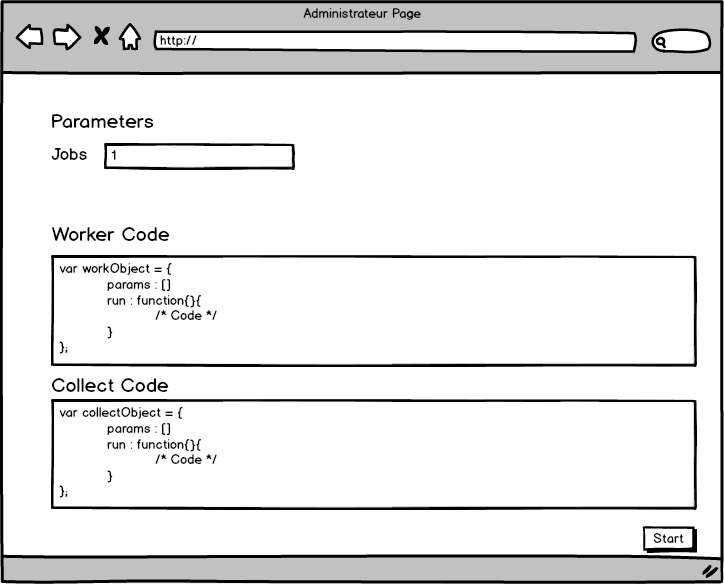
\includegraphics[width=0.9\textwidth]{IntChercheur.png}
\end{center}

\section{Technique}

La plateforme gére des calcul distribué qui seront fait en Javascript, pour cela on a opté pour le Javascript dans le coté serveur a fin qu'il y une compatibilité entre langages Front-end et Back-end. La plateforme utilise les technologies suivantes :

\begin{itemize}
\item Back-end : On utilise NodeJS comme serveur web, ensuite Express qui est un framework qui permet de déveloper des application web en Javascript plus rapidement, il permet aussi de gérer les routes URL ainsi que les requetes HTTP/HTTPS.
\item Front-end : les interfaces chercheur et volontaire sont conçus en HTML/Javascript/CSS, pour l'interface Chercheur les communication sont faite en HTTP, parcontre dans l'interface Volontaire la premier requete pour se rendre sur le site de la plateforme se fait par HTTP classic, puis pour toute les communication prochaines en bascule vers les websockets.
\item Middleware : L'utilisation d'un middleware type serveur de file de messages, ce serveur permetteras de stocker les jobs créer, et aussi les résultats des jobs reçus de la part des volontaires, il permettra aussi d'avoir une bonne scalabilité de notre application en ayant la possibilité d'ajouter des instance du serveur web pour augmenter les performances de la plateforme.
\end{itemize} 

\begin{figure}[h]
\centering
\includegraphics[width=1\textwidth]{ArchGen.png}
\caption{\label{fig:ArchGenarale}Architecture générale de la plate-forme}
\end{figure}

\section{Scénarios}
\subsection{scénario lancement du calcul}

\subsection{scénario creation/envoie des jobs}
\subsection{scénario récuperation des résultats}

\end{document}

